\documentclass[11pt]{article}

\usepackage[utf8]{inputenc}
\usepackage[T1]{fontenc}
\usepackage[margin=1in]{geometry}
\usepackage{graphicx}
\usepackage{booktabs}
\usepackage{amsmath}
\usepackage{amssymb}
\usepackage{url}
\usepackage{natbib}
\usepackage[hidelinks]{hyperref}
\usepackage{caption}

\captionsetup{font=small,labelfont=bf}

\title{\textbf{The Informational Diet of /pol/}\\[0.3em]
\large A citation-level audit of source use and discourse tone\\
across 278{,}706 posts on 4chan's Politically Incorrect board}

\author{Marc Garnier\thanks{Correspondence: \texttt{garniermarc.pro@gmail.com}.
Code and derived data: \url{https://github.com/marcgarnier/4chan-pol-source-audit}.}}

\date{September 4, 2026}

\begin{document}
\maketitle

\begin{abstract}
\noindent
Research on 4chan's /pol/ board routinely frames its information environment as a
contest between mainstream and alternative news media. We test that framing
empirically. Over 24 daily captures spanning 45 days (2026-07-22 to 2026-09-04) we
collected 6{,}532 threads and 278{,}706 posts, extracted every external URL, and
coded 10{,}078 citation events across 1{,}408 unique domains, attaching a
transformer sentiment score to the discussion surrounding each citation.

The framing does not survive contact with the data. News outlets of any
kind---mainstream, alternative, and state-controlled combined---account for
\textbf{4.6\%} of citation events. What /pol/ actually circulates is
platform content (40.3\%) and a long, largely unclassifiable tail (47.2\%),
of which file hosts and archives are a substantial and behaviourally
meaningful component (9.2\% of all citations). Sourcing is extremely
concentrated: a Gini coefficient of 0.821, with YouTube alone supplying
28.9\% of citations and twelve domains supplying half.

Discourse tone differs across source categories (Kruskal--Wallis $H=110.0$,
$p<10^{-21}$), but the effect is substantively small ($\varepsilon^2=0.011$;
adjusted $R^2=0.067$). Mainstream citations sit in measurably more negative
discussion than platform, unclassified, or institutional citations
(Cliff's $\delta$ between 0.21 and 0.26, all $p_{\text{Holm}}<10^{-7}$).
The specific mainstream-versus-alternative contrast that motivates the
literature, however, is \textbf{not supported}: $p_{\text{Holm}}=0.83$,
$\delta=-0.121$ (negligible), with $n=69$ alternative citations affording
essentially no power.

We also convert the design's primary validity threat into a measurement.
Across 62 pairs of repeated thread captures, 0.68\% of posts
(95\% CI [0.44, 1.07]) disappeared between observations---a bound that is
itself conditioned on thread survival and therefore a floor, not an estimate.
We argue that the mainstream/alternative frame is the wrong instrument for
this object, and that platform and archive infrastructure is the more
defensible unit of analysis.
\end{abstract}

\section{Introduction}

4chan's /pol/ (``Politically Incorrect'') board occupies an outsized place in
accounts of online radicalisation and information disorder. Measurement work
has characterised its language, its raiding behaviour, and its position in the
wider web ecosystem \citep{hine2017,papasavva2020}. A recurring assumption in
this literature, and in journalistic accounts drawing on it, is that /pol/
constitutes an \emph{alternative media ecosystem}: a space where legacy outlets
are rejected and replaced by a counter-canon of partisan publishers.

That assumption is rarely measured directly. It requires knowing what /pol/
cites, in what proportion, and how the surrounding discussion treats each kind
of source. This paper supplies that measurement for a bounded collection window
and reports a result that is largely negative for the framing.

Our contributions are four:

\begin{enumerate}
\item \textbf{A citation-level audit.} 10{,}078 citation events over 45 days,
coded by medium type, with proportions reported as Wilson score intervals.
\item \textbf{A concentration analysis.} Gini, normalised HHI, and a Lorenz
curve over the domain distribution, quantifying how narrow the diet is.
\item \textbf{An inferential test of the tone hypothesis} with effect sizes and
a thread-clustered adjusted model---including an explicit null on the
mainstream/alternative contrast.
\item \textbf{A measured bound on survivorship bias}, derived from repeated
captures of the same threads, in place of the usual qualitative caveat.
\end{enumerate}

\section{Related work}

\citet{hine2017} provided the first large-scale measurement of /pol/,
characterising its posting dynamics, its hate-speech prevalence, and its
raiding of other platforms. \citet{papasavva2020} released a 3.5-year corpus of
augmented /pol/ posts, establishing the dataset conventions much subsequent
work relies on. Both establish /pol/ as an object of quantitative study; neither
takes the citation event as the unit of analysis.

Source-classification work in computational social science generally anchors
labels to third-party rating databases rather than author judgment---AllSides,
Media Bias/Fact Check, and Ad Fontes are the common choices
\citep{bozarth2020,robertson2018}. We adopt that principle, with the
substantial caveat noted in Section~\ref{sec:limits}: our present
implementation codes only the medium-type axis, and the ratings-anchored
orientation and ownership axes remain specified but unimplemented.

For sentiment we use the TweetEval RoBERTa model
\citep{barbieri2020,loureiro2022}. Its limitations on this domain are
substantial and we treat them as a first-order threat rather than a footnote
(Section~\ref{sec:limits}).

\section{Data and methods}

\subsection{Collection}

Threads were captured from the live /pol/ JSON API via the 4TCT
collector on a daily cadence, yielding 24 daily captures between
2026-07-22 and 2026-09-04. This is a \emph{snapshot} design: conclusions
are scoped to the collection window, not to /pol/ in general or across time.

\begin{table}[t]
\centering
\small
\begin{tabular}{lr}
\toprule
Threads captured & 6{,}532 \\
Posts & 278{,}706 \\
Posts with $\geq 1$ external link & 7{,}107 (2.55\%) \\
Citation events & 10{,}078 \\
Unique domains & 1{,}408 \\
Daily captures & 24 \\
Window & 2026-07-22 -- 2026-09-04 \\
\bottomrule
\end{tabular}
\caption{Corpus summary.}
\label{tab:corpus}
\end{table}

\subsection{Citation extraction and unit of analysis}

The unit of analysis is the \textbf{citation event}: one external domain
appearing in one post. Posts may contain several distinct domains; each is
counted once per post, deduplicated within the post. Links internal to 4chan
are excluded. Mobile and shortened hosts are normalised to a canonical domain
(\texttt{youtu.be}, \texttt{m.youtube.com} $\rightarrow$ \texttt{youtube.com}),
and subdomain matching resolves cases such as \texttt{en.wikipedia.org}.

We note that an earlier version of our pipeline retained only the first domain
per post and discarded the remainder. Because /pol/ posts characteristically
lead with a video or tweet and append a source, this systematically discarded
the appended source: alternative-media citations were undercounted by a factor
of 3.6 (19 recorded against 69 actual). All figures reported here use
per-citation counting, and we flag the failure mode because it is a plausible
silent defect in any pipeline that treats a post as carrying one source.

\subsection{Source coding}

Domains are coded on the \emph{medium type} axis by deterministic rules:
institutional/reference (Wikimedia family; \texttt{.gov}, \texttt{.mil},
\texttt{.edu} by suffix); social platform (curated platform set); news outlet,
subdivided into mainstream, alternative, and state-controlled; and unclassified.
Section~\ref{sec:limits} states plainly what this coding does and does not
license.

\subsection{Sentiment measurement}

Each post carrying at least one citation is scored with
\texttt{cardiffnlp/twitter-roberta-base-sentiment-latest}
\citep{barbieri2020,loureiro2022}. The three-way softmax is collapsed to a
compound score in $[-1,+1]$ as $s = p_{\text{pos}} - p_{\text{neg}}$. A post is
scored once; the score is attached to each of its citation events.

Critically, the score is computed over the \emph{entire post}. It measures the
\textbf{ambient tone of discussion surrounding a citation}, not the author's
stance toward the cited source. ``CNN is garbage, here's proof'' yields a
negative score attached to CNN even though the poster is endorsing the link's
content. Every tone result below must be read under that construct definition.

\subsection{Statistical analysis}

Proportions are reported with 95\% Wilson score intervals \citep{wilson1927},
which behave correctly for the small and extreme cells this distribution
produces. Concentration is measured by the Gini coefficient and a normalised
Herfindahl--Hirschman index over per-domain citation counts.

For tone we use Kruskal--Wallis \citep{kruskal1952} as the omnibus test---the
sentiment distribution is bounded and non-normal---with $\varepsilon^2$ as the
effect size, followed by Dunn post-hoc tests with tie correction and Holm
step-down adjustment \citep{holm1979}. Pairwise effect sizes are Cliff's
$\delta$ \citep{cliff1993}, interpreted at the conventional thresholds
(negligible $<0.147$, small $<0.33$, medium $<0.474$). We report effect sizes
throughout: at $n=10{,}078$, statistical significance is cheap and carries
little substantive information on its own.

The adjusted model is an OLS regression of compound sentiment on source
category, thread topic, and $\log(1+\text{post length})$, with standard errors
clustered by thread, since citations within a thread are not independent.

\section{Results}

\subsection{What /pol/ cites}

Figure~\ref{fig:main}(a) and Table~\ref{tab:shares} give the distribution.
The result that organises everything else: \textbf{news outlets of any
description account for 4.6\% of citation events}. Mainstream outlets supply
3.8\% [3.5, 4.2], alternative outlets 0.7\% [0.5, 0.9], and state-controlled
outlets 0.1\% [0.1, 0.2]. Social platforms supply 40.3\%, and 47.2\% of
citations fall outside any of these categories.

\begin{figure}[t]
\centering
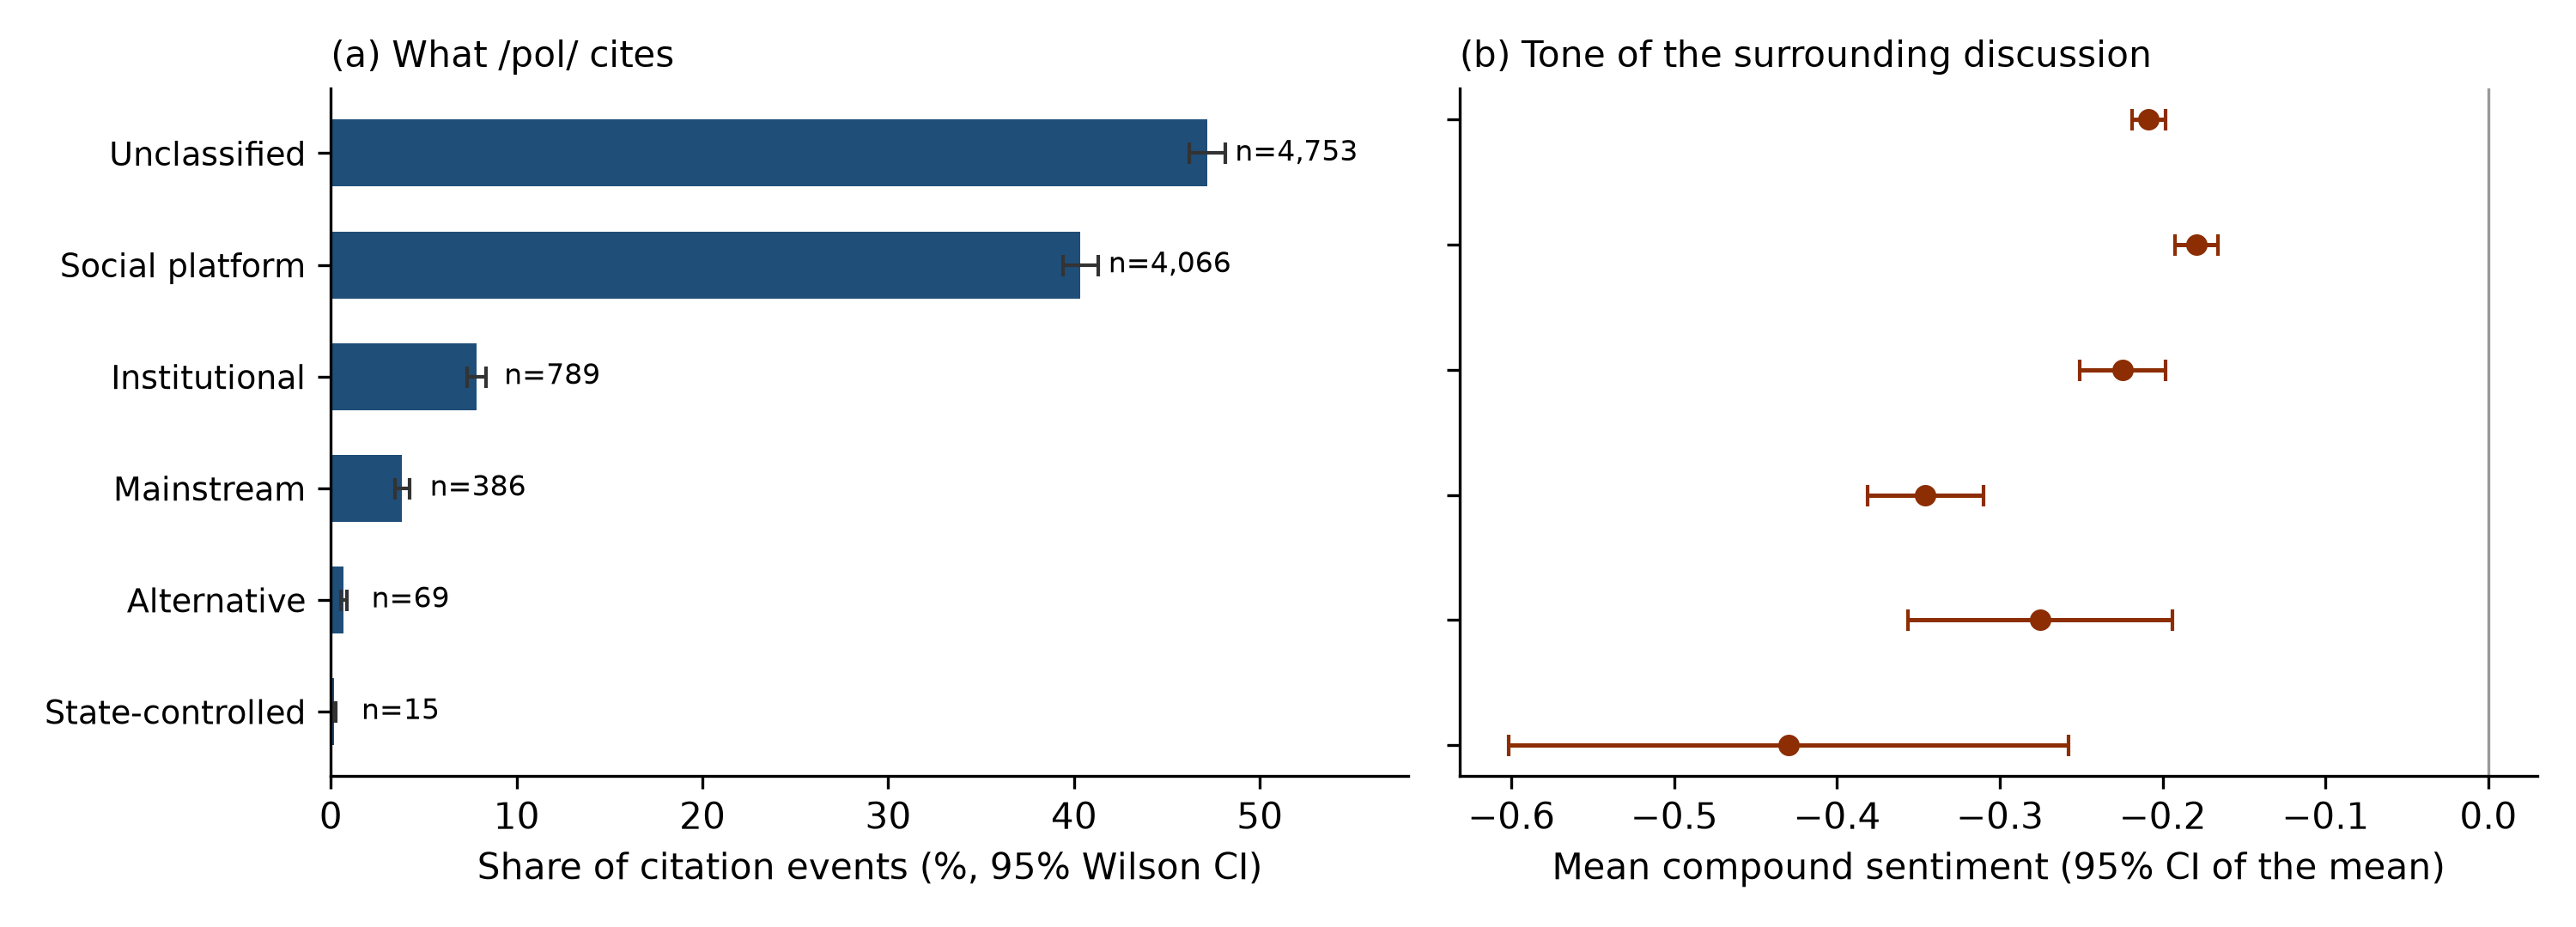
\includegraphics[width=\textwidth]{fig_main.png}
\caption{(a) Share of citation events by source category, with 95\% Wilson
score intervals. (b) Mean compound sentiment of the surrounding discussion,
with 95\% confidence intervals \emph{of the mean}. The width of the Alternative
and State-controlled intervals in (b) is the whole story of the null result in
Section~\ref{sec:tone}.}
\label{fig:main}
\end{figure}

\begin{table}[t]
\centering
\small
\begin{tabular}{lrrrrr}
\toprule
Category & $n$ & Share & 95\% CI & Mean sent. & Neg. ratio \\
\midrule
Unclassified      & 4{,}753 & 47.2\% & [46.2, 48.1] & $-0.209$ & 46.5\% \\
Social platform   & 4{,}066 & 40.3\% & [39.4, 41.3] & $-0.179$ & 39.4\% \\
Institutional     & 789     & 7.8\%  & [7.3, 8.4]   & $-0.225$ & 45.2\% \\
Mainstream        & 386     & 3.8\%  & [3.5, 4.2]   & $-0.346$ & 66.1\% \\
Alternative       & 69      & 0.7\%  & [0.5, 0.9]   & $-0.275$ & 62.3\% \\
State-controlled  & 15      & 0.1\%  & [0.1, 0.2]   & $-0.430$ & 86.7\% \\
\bottomrule
\end{tabular}
\caption{Citation events by source category. ``Neg.\ ratio'' is the share of
citations whose surrounding post scores below $-0.2$.}
\label{tab:shares}
\end{table}

These proportions are stable across the window. Daily mainstream share ranges
from 1.8\% to 6.0\% (median 3.7\%) and daily platform share from 33.5\% to
51.5\% (median 40.4\%) across the 24 captures, with no visible trend.

\subsection{Concentration}

The diet is not merely non-journalistic; it is narrow.
The domain distribution has a Gini coefficient of \textbf{0.821} and a
normalised HHI of 0.091. YouTube alone supplies \textbf{28.9\%} of all citation
events; the top ten domains supply 49.1\% and the top fifty 69.0\%. Twelve
domains account for half of all citations. At the other end, 989 of 1{,}408
domains (70.2\%) appear exactly once. Figure~\ref{fig:lorenz} plots the Lorenz
curve.

\begin{figure}[t]
\centering
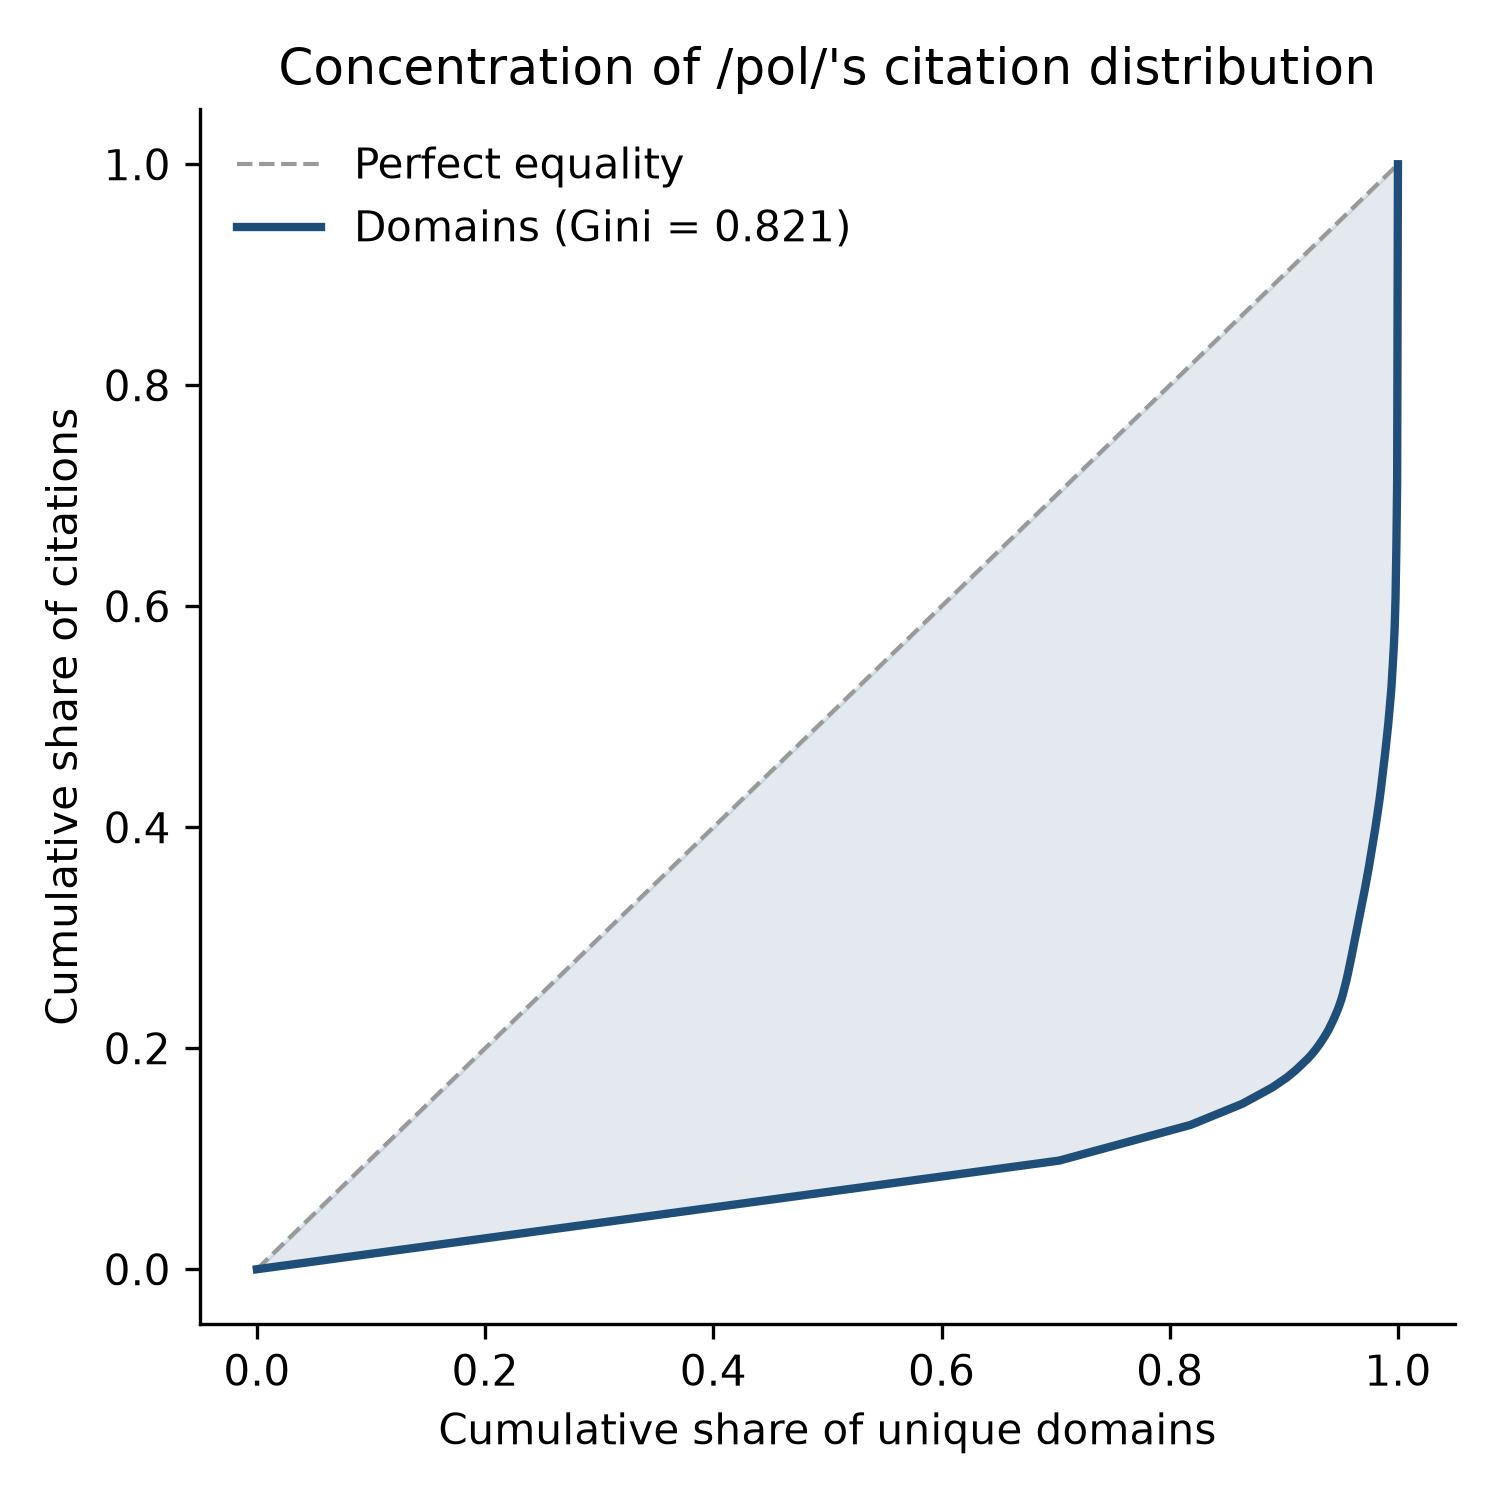
\includegraphics[width=0.52\textwidth]{fig3_lorenz.png}
\caption{Lorenz curve of the citation distribution over 1{,}408 unique domains.}
\label{fig:lorenz}
\end{figure}

\subsection{Archives and file hosts are a sourcing behaviour}

The 47.2\% ``unclassified'' bucket is not homogeneous noise. File hosts and
archiving services account for \textbf{928 citation events}---9.2\% of all
citations and 19.5\% of the unclassified bucket. The leading members are
\texttt{files.catbox.moe} (253), \texttt{rentry.org} (168),
\texttt{archive.4plebs.org} (117), \texttt{archive.today} (83),
\texttt{archive.ph} (66) and \texttt{archive.is} (63).

Read as infrastructure rather than residue, this is a coherent practice:
hosting media outside platform moderation, and preserving content---including
4chan's own deleted threads, via 4plebs---against removal. On this board,
archive use is roughly \emph{twice} as frequent as citing mainstream news.

\subsection{Discourse tone by source category}
\label{sec:tone}

Tone differs across categories: Kruskal--Wallis $H=110.0$, $p=4.0\times
10^{-22}$. The effect size, however, is $\varepsilon^2=0.011$---source category
accounts for roughly one percent of the variance in sentiment. The adjusted
model reaches $R^2=0.067$. Whatever is driving tone on /pol/, the category of
the cited source is a minor part of it.

Table~\ref{tab:posthoc} gives the post-hoc structure. Mainstream citations sit
in reliably more negative discussion than platform ($\delta=0.255$),
unclassified ($\delta=0.242$), and institutional ($\delta=-0.208$) citations,
all at small effect magnitude and all surviving Holm correction comfortably.

\begin{table}[t]
\centering
\small
\begin{tabular}{lrrrl}
\toprule
Contrast & $z$ & $p_{\text{Holm}}$ & Cliff's $\delta$ & Magnitude \\
\midrule
Social platform vs.\ Mainstream       & 9.24  & $<10^{-15}$        & 0.255  & small \\
Unclassified vs.\ Mainstream          & 7.10  & $1.8\times10^{-11}$& 0.242  & small \\
Mainstream vs.\ Institutional         & $-5.98$ & $2.9\times10^{-8}$ & $-0.208$ & small \\
Social platform vs.\ Unclassified     & 5.44  & $6.4\times10^{-7}$ & 0.070  & negligible \\
Social platform vs.\ Institutional    & 3.09  & 0.022              & 0.067  & negligible \\
Social platform vs.\ Alternative      & 2.88  & 0.040              & 0.181  & small \\
Social platform vs.\ State-controlled & 2.84  & 0.041              & 0.368  & medium \\
\midrule
\textbf{Mainstream vs.\ Alternative}  & $-1.09$ & \textbf{0.827}   & $-0.121$ & negligible \\
\bottomrule
\end{tabular}
\caption{Dunn post-hoc contrasts with Holm correction, ordered by adjusted
$p$. All contrasts above the rule are significant at $\alpha=0.05$; the
contrast below it is the one the literature's framing predicts, and it is not.
Contrasts omitted for space were all non-significant.}
\label{tab:posthoc}
\end{table}

\paragraph{The central contrast is null.}
Mainstream versus alternative---the comparison the alternative-ecosystem
framing predicts---yields $z=-1.09$, $p_{\text{Holm}}=0.827$, and
$\delta=-0.121$, a negligible magnitude. The raw means differ in the predicted
direction ($-0.346$ against $-0.275$), and reporting that difference without a
test would have produced a confident and false headline. With $n=69$
alternative citations, the study has essentially no power to resolve a gap of
this size, and we decline to interpret it.

The adjusted model (Table~\ref{tab:model}) reproduces this pattern. Relative to
social platforms, mainstream citations carry $-0.094$ ($p=1.6\times10^{-5}$)
and state-controlled citations $-0.218$ ($p=0.026$), while alternative
citations are statistically indistinguishable from platform citations
($\beta=-0.008$, $p=0.86$). Post length is a stronger and more reliable
predictor than most category contrasts: each unit of $\log$ length carries
$-0.042$ ($p=1.2\times10^{-14}$). Longer posts are angrier posts.

\begin{table}[t]
\centering
\small
\begin{tabular}{lrrr}
\toprule
Term & $\beta$ & SE & $p$ \\
\midrule
Intercept                        & 0.033   & 0.086 & 0.70 \\
Mainstream                       & $-0.094$& 0.022 & $1.6\times10^{-5}$ \\
State-controlled                 & $-0.218$& 0.098 & 0.026 \\
Institutional                    & $-0.020$& 0.015 & 0.18 \\
Alternative                      & $-0.008$& 0.045 & 0.86 \\
Unclassified                     & 0.006   & 0.011 & 0.57 \\
Topic: Elections / Politics      & 0.239   & 0.084 & 0.004 \\
$\log(1+\text{post length})$     & $-0.042$& 0.005 & $1.2\times10^{-14}$ \\
\bottomrule
\end{tabular}
\caption{OLS regression of compound sentiment, standard errors clustered by
thread ($n=10{,}078$ citations in 2{,}642 threads; $R^2=0.067$). Reference
category is social platform; reference topic is Economy / Finance. Remaining
topic terms omitted for space.}
\label{tab:model}
\end{table}

\subsection{Co-citation structure}

Domains co-occurring within a thread form a weighted graph (edges with weight
$\geq 2$): 286 nodes, 1{,}846 edges, density 0.045. Louvain community detection
yields six communities at modularity 0.429. The largest (198 domains) is a
general-purpose cluster anchored on YouTube, Wikipedia, and mainstream outlets;
smaller ones are topical---a war-tracking cluster
(\texttt{liveuamap}, \texttt{marinetraffic}, \texttt{vesselfinder},
\texttt{oilprice}), a US-politics platform cluster
(\texttt{twitter}, \texttt{truthsocial}, \texttt{rumble}), and a German-language
cluster. Sourcing ecosystems on /pol/ appear organised by topic and by
platform affordance, not by editorial orientation.

\subsection{A measured bound on survivorship}
\label{sec:deletion}

Sixty-two pairs of repeated captures of the same thread let us measure directly
what is usually asserted: \textbf{19 of 2{,}776 observed posts (0.68\%,
95\% CI [0.44, 1.07]) had disappeared by the following capture}, affecting 7 of
the paired threads.

This number must be read for what it is. It measures post-level deletion
\emph{within threads that survived to be captured twice}. It says nothing about
threads deleted in their entirety, nor about threads born and died between two
daily captures---which, at a daily cadence on a board with /pol/'s velocity, is
the larger loss channel. It is therefore a \textbf{floor on content loss, not
an estimate of it}, and it is a floor derived from a self-selected sample. We
report it because a measured floor is more useful than an unmeasured caveat,
not because it settles the question.

\section{Discussion}

\paragraph{The frame does not fit the object.}
A research literature that asks whether /pol/ prefers alternative to mainstream
media is asking about 4.6\% of what /pol/ circulates. The board's information
diet is overwhelmingly platform-mediated and archive-supported: a YouTube link
with commentary, a Telegram forward, a catbox-hosted image, a 4plebs permalink
to a deleted thread. Treating this as a \emph{news} ecosystem---counter or
otherwise---imports a print-era category that the object does not honour. The
more defensible unit is platform and archival infrastructure.

\paragraph{Significance is not magnitude.}
Category differences in tone are real and, on the well-populated categories,
robust. They are also small: one percent of sentiment variance. A study of this
size can detect almost anything; reporting $p$-values without $\varepsilon^2$
and $\delta$ would have dressed a marginal effect as a finding. The
mainstream/alternative null is the sharper lesson---the difference sits in the
predicted direction and would have been reported as confirmation by any
analysis that stopped at group means.

\paragraph{What negativity toward mainstream citations does and does not mean.}
Mainstream citations reliably attract more negative surrounding discourse. Under
our construct definition this is ambient tone, not stance. Both readings are
consistent with it: hostility to the outlet, and hostility to the \emph{event}
that mainstream outlets disproportionately report. We cannot separate them
without target-dependent stance detection \citep{mohammad2016,pontiki2016}, and
we do not claim to.

\section{Limitations}
\label{sec:limits}

We state these at full strength; several are severe enough to bound what the
paper can claim.

\paragraph{Sentiment measurement is unvalidated on this domain.}
The model was trained on Twitter. /pol/'s irony, slang, and toxicity are
out-of-distribution, and we have \emph{not} performed the human-annotated
validation that would quantify the resulting measurement error. Every tone
result in Section~\ref{sec:tone} should be treated as provisional pending a
hand-coded sample of 100--200 posts with reported model--human agreement. The
descriptive and concentration results (Sections 4.1--4.3) do not depend on the
sentiment model and are unaffected.

\paragraph{Source coding is single-axis and partially unanchored.}
Our design calls for coding each domain on three orthogonal axes---medium type,
editorial orientation, and ownership/control---against external rating
databases (AllSides, MBFC, Ad Fontes, RSF), precisely because forcing them into
one label is what makes cases like Fox News, BBC, and France 24 irreconcilable.
The implementation reported here codes only the medium-type axis, and its
news-outlet subdivision into mainstream/alternative/state-controlled is a
curated list, not a ratings-anchored mapping. No inter-annotator agreement was
computed. The mainstream/alternative/state distinctions therefore carry lower
construct validity than the platform, institutional, and archive distinctions,
which rest on deterministic structural rules.

\paragraph{Survivorship bias is bounded below, not corrected.}
See Section~\ref{sec:deletion}. Moderation on /pol/ removes the most extreme
content preferentially, so the surviving corpus is a filtered view---filtered
in the direction of the phenomenon being measured. Source-distribution
estimates are relatively robust to this, since deletion would need to correlate
with the category of the cited source. Tone estimates are directly exposed,
because deletion correlates with discourse extremity, which is what the
sentiment score captures.

\paragraph{Small cells preclude inference.}
$n=69$ (alternative) and $n=15$ (state-controlled) support description only. No
amount of additional collection fixes this efficiently: at 0.7\% and 0.1\% of
citations, reaching usable power would require an order of magnitude more data
or a broader ratings-anchored domain list. The latter is the correct fix.

\paragraph{Topic classification is weak.}
Thread topics are assigned by keyword matching over the opening post's subject
and slug. 76.2\% of posts fall into ``Other / Misc''. The topic covariate in
Table~\ref{tab:model} should be read as a coarse control, not as a
substantive topical analysis.

\paragraph{Scope.}
One board, 24 daily captures, 45 days. Results describe the surviving, publicly
visible discourse of /pol/ during that window. They do not generalise to /pol/
across time, nor to other imageboards.

\section{Conclusion}

/pol/ is not primarily arguing about the news. It is circulating platform media
and archived artefacts, with legacy and alternative outlets together occupying
under five percent of its citation stream and a handful of domains dominating
the rest. Where tone does differ by source category, the differences are
statistically clear but substantively small, and the one contrast the field's
framing most confidently predicts---mainstream against alternative---does not
reach significance at the sample size the board itself affords.

The productive move is not more data under the same frame. It is to take
platform and archive infrastructure as the unit of analysis, to anchor source
coding to external rating databases across all three axes, and to replace
whole-post sentiment with target-dependent stance detection. All three are
tractable; none of them are what the current framing asks for.

\section*{Data and code availability}

Analysis code, derived statistics, and figures are available at
\url{https://github.com/marcgarnier/4chan-pol-source-audit}. The raw capture
corpus (\textasciitilde 600\,MB) is not redistributed; it is reproducible from the
public 4chan JSON API using the collection scripts provided. All results in this
paper are regenerated by \texttt{analysis.py} from the released database schema.

\begin{thebibliography}{99}

\bibitem[Barbieri et al.(2020)]{barbieri2020}
Barbieri, F., Camacho-Collados, J., Neves, L., \& Espinosa-Anke, L. (2020).
TweetEval: Unified Benchmark and Comparative Evaluation for Tweet
Classification. \emph{Findings of EMNLP 2020}.

\bibitem[Bozarth et al.(2020)]{bozarth2020}
Bozarth, L., Saraf, A., \& Budak, C. (2020). Higher Ground? How Groundtruth
Labeling Impacts Our Understanding of Fake News about the 2016 U.S.
Presidential Nominees. \emph{ICWSM 2020}.

\bibitem[Cliff(1993)]{cliff1993}
Cliff, N. (1993). Dominance statistics: Ordinal analyses to answer ordinal
questions. \emph{Psychological Bulletin}, 114(3), 494--509.

\bibitem[Hine et al.(2017)]{hine2017}
Hine, G. E., Onaolapo, J., De Cristofaro, E., Kourtellis, N., Leontiadis, I.,
Samaras, R., Stringhini, G., \& Blackburn, J. (2017). Kek, Cucks, and God
Emperor Machine Learning: A Measurement Study of 4chan's Politically Incorrect
Board. \emph{ICWSM 2017}.

\bibitem[Holm(1979)]{holm1979}
Holm, S. (1979). A simple sequentially rejective multiple test procedure.
\emph{Scandinavian Journal of Statistics}, 6(2), 65--70.

\bibitem[Kruskal \& Wallis(1952)]{kruskal1952}
Kruskal, W. H., \& Wallis, W. A. (1952). Use of ranks in one-criterion variance
analysis. \emph{Journal of the American Statistical Association}, 47(260),
583--621.

\bibitem[Loureiro et al.(2022)]{loureiro2022}
Loureiro, D., Barbieri, F., Neves, L., Espinosa-Anke, L., \& Camacho-Collados,
J. (2022). TimeLMs: Diachronic Language Models from Twitter. \emph{ACL 2022,
System Demonstrations}.

\bibitem[Mohammad et al.(2016)]{mohammad2016}
Mohammad, S., Kiritchenko, S., Sobhani, P., Zhu, X., \& Cherry, C. (2016).
SemEval-2016 Task 6: Detecting Stance in Tweets. \emph{SemEval 2016}.

\bibitem[Papasavva et al.(2020)]{papasavva2020}
Papasavva, A., Zannettou, S., De Cristofaro, E., Stringhini, G., \& Blackburn,
J. (2020). Raiders of the Lost Kek: 3.5 Years of Augmented 4chan Posts from the
Politically Incorrect Board. \emph{ICWSM 2020}.

\bibitem[Pontiki et al.(2016)]{pontiki2016}
Pontiki, M., Galanis, D., Papageorgiou, H., et al. (2016). SemEval-2016 Task 5:
Aspect-Based Sentiment Analysis. \emph{SemEval 2016}.

\bibitem[Robertson et al.(2018)]{robertson2018}
Robertson, R. E., Jiang, S., Joseph, K., Friedland, L., Lazer, D., \& Wilson, C.
(2018). Auditing Partisan Audience Bias within Google Search. \emph{CSCW 2018}.

\bibitem[Wilson(1927)]{wilson1927}
Wilson, E. B. (1927). Probable inference, the law of succession, and statistical
inference. \emph{Journal of the American Statistical Association}, 22(158),
209--212.

\end{thebibliography}

\end{document}
